\documentclass[11pt]{article}
\usepackage{mypackages}
\begin{document}

\section{Results}

For each of the experiments described in the previous section, we will be comparing the
scores achieved to the amount of \textit{timesteps} completed in the experiments.
The timestep is increased every time an action is performed and a new state is encountered.
For the CartPole problem we will be using the timesteps completed as a constraint for
how long the experiments are allowed to run.
This approach makes it more fair for each thread setting, as we expect 
that we should be able to complete more timesteps using the same amount of real time
with multiple threads.

In the experiments testing the A3C method on Atari games, using timesteps as a constraint
was not an option, due to the amount of real time it would require, for especially the lower thread settings.
Therefore all of these experiments have only been allowed to run for 16 hours,
due to the time and resource limitations of this project.

\subsection{Playing CartPole - Actor-Critic with eligibility traces}

For this experiment our implementation was allowed to take at most 200.000 timesteps.
The pace of learning depends on the experience obtained during exploration.
Therefore we ran the experiment five times to show the average performance of
the implementation.
In figure \ref{fig:cp_et} the results of the experiment is shown
as a function of real-time(\ref{fig:cp_et_t}) and timesteps(\ref{fig:cp_et_ts}).
The Actor-Critic method with eligibility traces is a single-threaded
approach and therefore the plots should roughly show the same tendency.

\begin{figure}[H]
    \begin{tabular}[c]{c}
    \begin{subfigure}{\textwidth}
        \centering
        \fbox{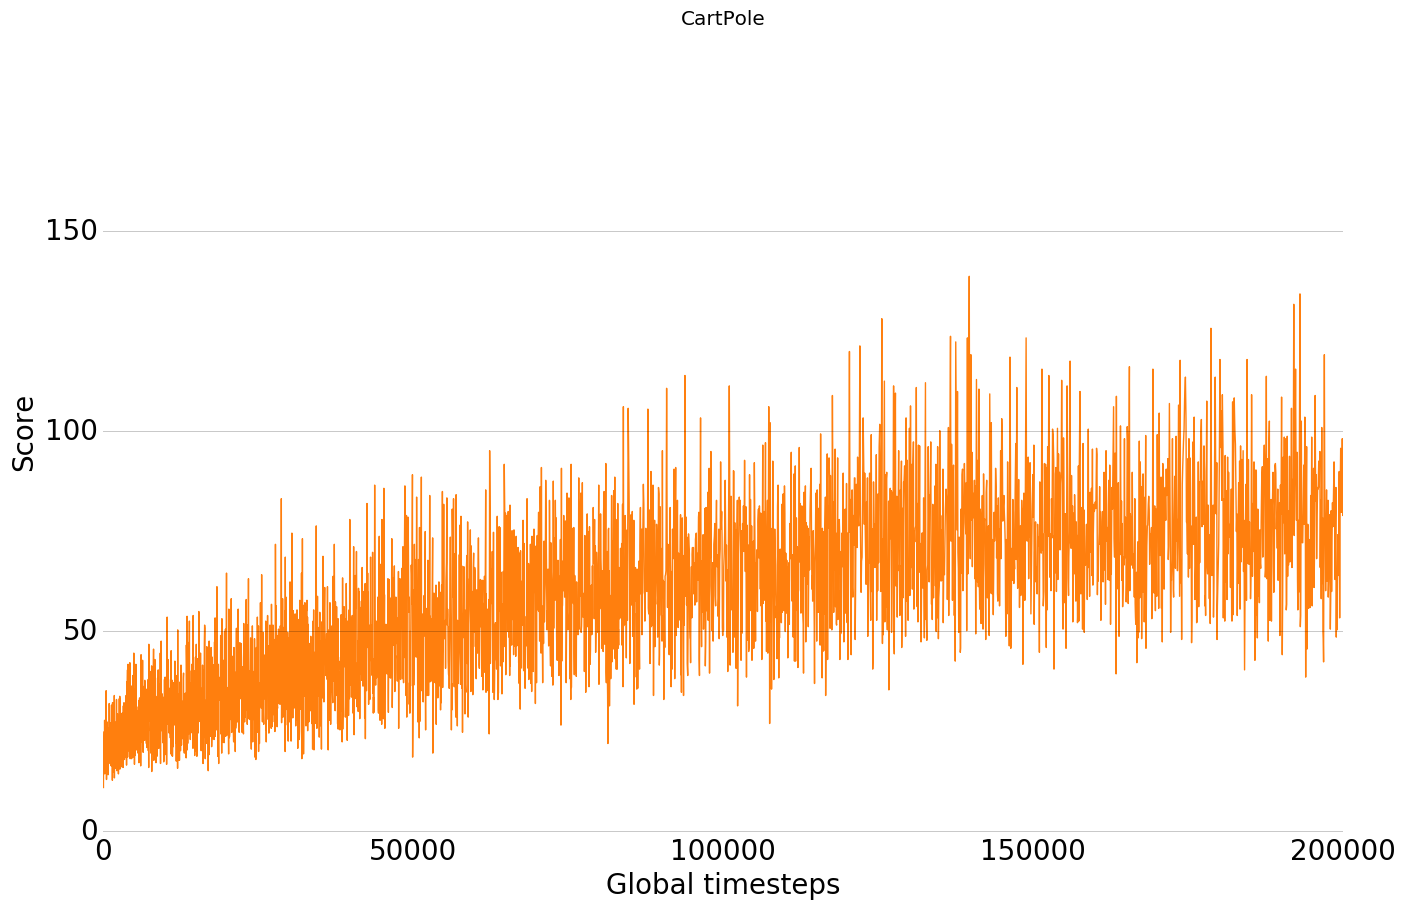
\includegraphics[scale=0.4]{plots/eligibility_steps.png}}
        \caption{The score of the Actor-Critic method with eligibility
            traces as a function of the number of timesteps
            the algorithm have been running.}
            \label{fig:cp_et_ts}
    \end{subfigure}
    \end{tabular}
    \begin{tabular}[c]{c}
    \begin{subfigure}{\textwidth}
        \centering
        \fbox{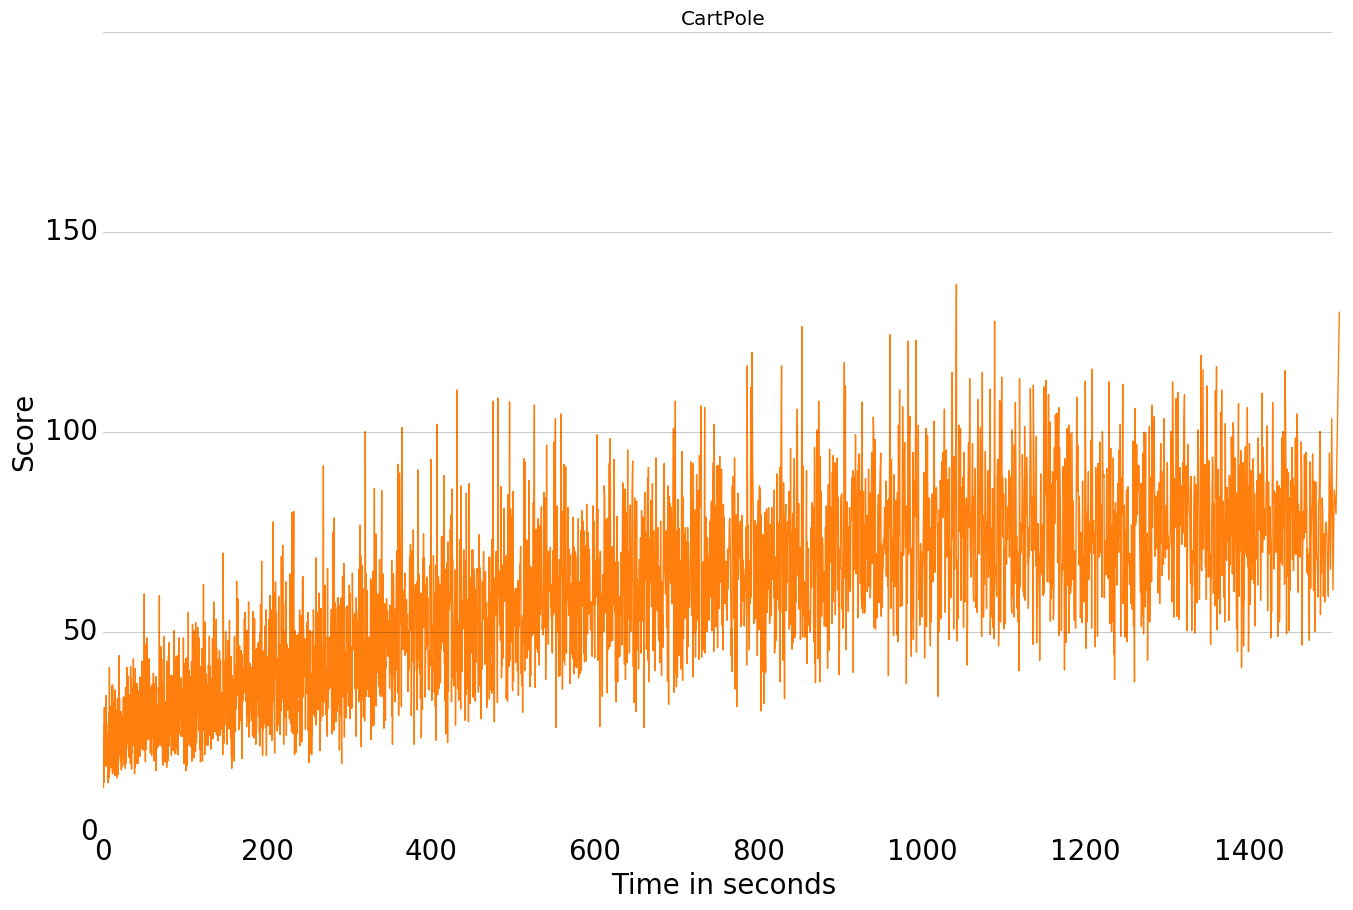
\includegraphics[scale=0.415]{plots/eligibility_time.png}}
        \caption{The score of the Actor-Critic method with eligibility
            traces as a function of the time in seconds the algorithm
            have been running.}
        \label{fig:cp_et_t}
    \end{subfigure}
    \end{tabular}
    \caption{Average results of five runs of the CartPole experiment using the Actor-Critic method
    with eligibility traces.} 
     \label{fig:cp_et}
\end{figure}

Unlike the Atari games, CartPole can be won if the player reaches a score of 200.
The results of our experiments suggest that
the method isn't able to learn how to solve the game completely,
since the highest mean score is 138,8, which is achieved after 139.688 timesteps.
However, the fact that the score increases over time
shows that it was able to learn how to play the game -
but not in most the optimal way.
This result reinforces the hypothesis that the implementation of the
Actor-Critic method with eligibility traces is suboptimal, even
though the average mean increased over the course of the experiment.
It is nonetheless notable that the method seems stable, in the sense that once it has learned
a policy it won't exchange it for a new policy that produces a significantly worse result.


\subsection{Playing CartPole - A3C}

In this experiment we also allowed the implementation to run for
200.000 timesteps.
Again the experiment was run five times to avoid lucky, and unlucky, runs
producing misleading results.
Figure \ref{fig:a3c_time_steps} and \ref{fig:a3c_time} shows the average result of the experiments for all thread settings - that is 16 threads, 8 threads, 4 threads,
2 threads and 1 thread - in timesteps and time in seconds, respectively.
Due to the natural variance in the results, 
we have smoothed the plots such that each point represent the mean of the 50
surrounding points.
We have applied the smoothing to make the plots more readable,
but it also means most of the variance has been removed.

\begin{figure}[H]
    \centering
    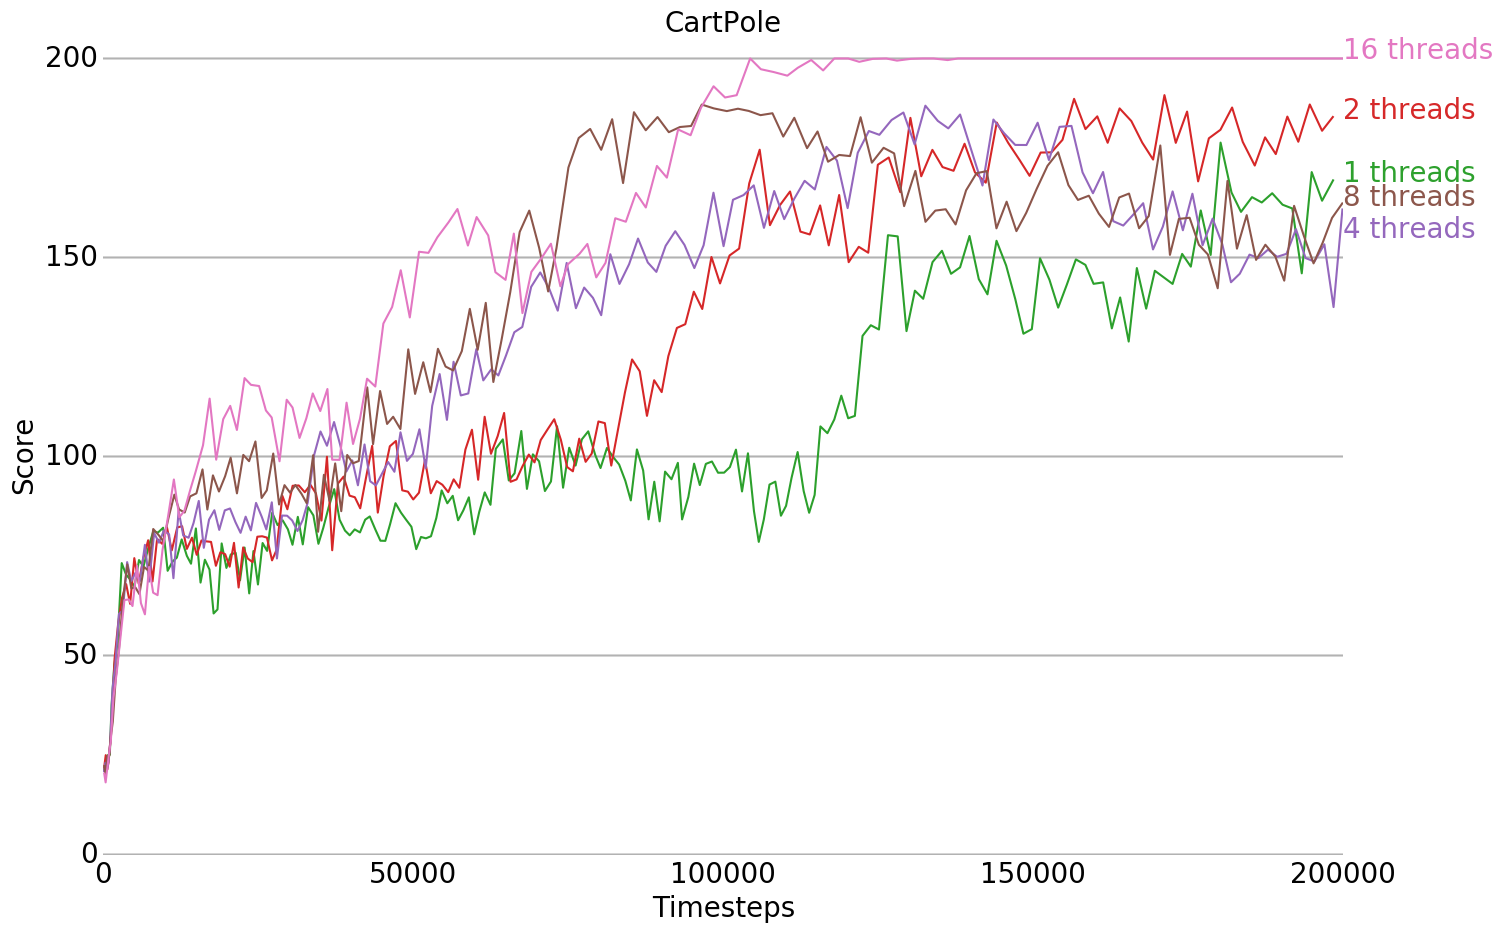
\includegraphics[scale=0.4]{plots/cartpole_compare_counter_without_AC.png}
    \caption{The score of the A3C method playing CartPole as a function
    of the number of timesteps the algorithm have been running.}
    \label{fig:a3c_time_steps}
\end{figure}

Looking at figure \ref{fig:a3c_time_steps}, it is clear that the
performance increases over time, as the policy improves.
The learning seems to happen in intervals which might suggest
that there exists certain thresholds in the game, where
suboptimal policies can still lead to decent scores.
Most of the learning seems to happen during the first 120.000 timesteps,
and afterwards the slope of the performance curve
is flattened until it has finished converging towards a mean score
of 200, which it does for the experiment using 16 threads.
It seems like the implementation is stable for all thread settings, with a slight
drop in performance after roughly half the timesteps using 8 threads.
However the drop is too insignificant to be classified as anything else than variance.
The overall result was not unexpected, as the same amount of timesteps should produce similar
scores regardless of the thread setting. 

\begin{figure}[H]
    \centering
    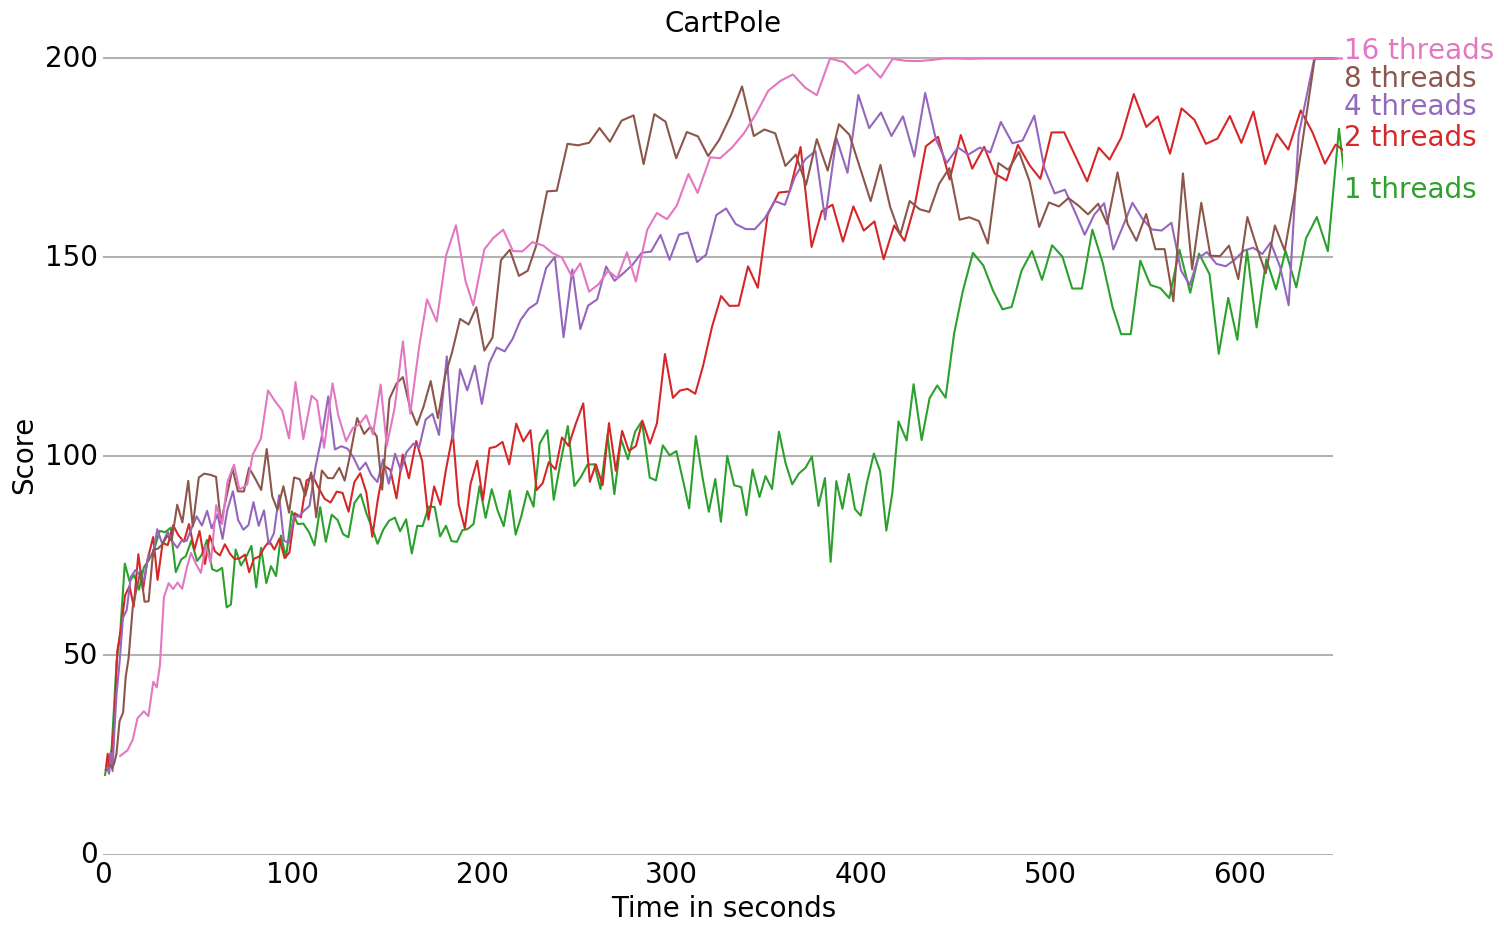
\includegraphics[scale=0.4]{plots/cartpole_compare_time_without_AC.png}
    \caption{The scores achieved by the A3C method playing CartPole as a function
    of the amount of time in seconds the algorithm have been running.
    Here the plot has been cut off after the first thread setting
    terminated.}
    \label{fig:a3c_time}
\end{figure}

Figure \ref{fig:a3c_time} shows the mean scores achieved over real time in seconds.
The plot has been cut off because the different thread settings didn't require the
same amount of time to complete 200.000 timesteps.
The time consumed can be more easily seen in table \ref{tab:time}, which shows that
the experiment using 8 threads was the first to complete all the timesteps.
It is unexpected that the experiment using 16 threads wasn't the first,
since a major advantage of the A3C method,
should be that using more threads should result in a higher amount of overall timesteps completed.
It is also notable that the plots of real-time and timesteps are almost identical
over all thread settings, which is surprising since the usage of more
threads didn't achieve a significant speedup
in time consumed by the implementation.
\begin{table}[H]
    \centering
 \begin{tabular}{ |l|c| }
  \hline
  \multicolumn{2}{|c|}{Median time spent completing 200.000 timesteps} \\
  \hline
  1 thread & 726,46 seconds \\
  \hline
  2 threads & 705,28 seconds \\
  \hline
  4 threads & 660,11 seconds \\
  \hline
  8 threads & 631,20 seconds \\
  \hline
  16 threads & 702,85 seconds \\
  \hline
 \end{tabular}
 \caption{The median time used to complete 200.000 timesteps
 for all thread settings over all the CartPole experiments using the A3C method.}
    \label{tab:time}
\end{table}


\subsubsection{Comparison between different amounts of threads}

Figure \ref{fig:a3c_comp_steps} shows the average result obtained from running 200.000
timesteps five times for each thread setting.

\begin{figure}[H]
  \centering   
  \begin{tabular}[c]{cc}
    \begin{subfigure}[c]{.5\textwidth}
        \fbox{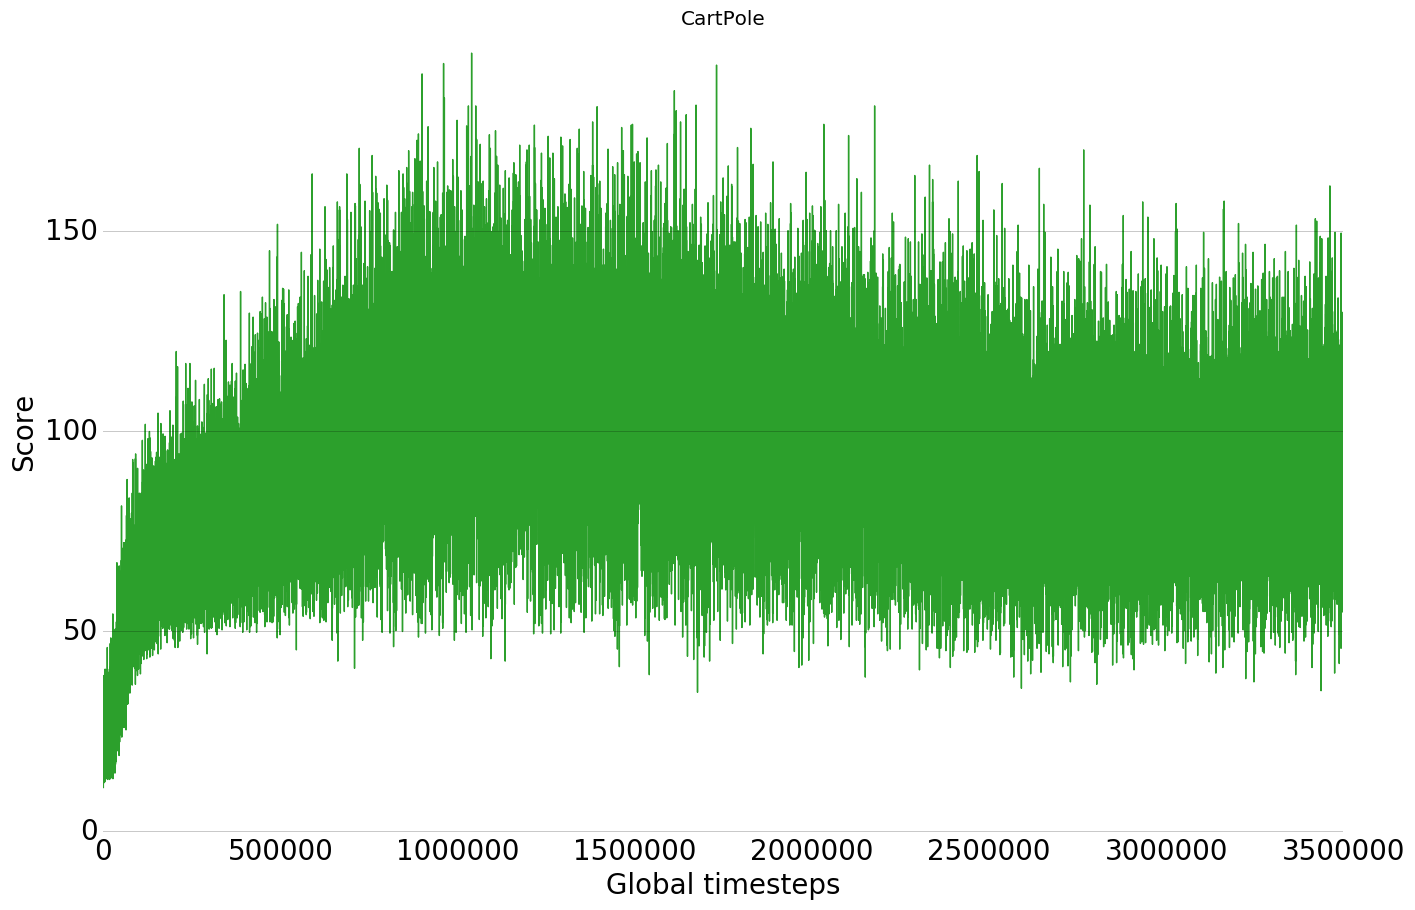
\includegraphics[width=0.95\textwidth]{plots/cartpole_1_threads.png}}
        \caption{A3C playing CartPole using 1 thread.}
        \label{cp:1}
    \end{subfigure}
    \begin{subfigure}[c]{.5\textwidth}
        \fbox{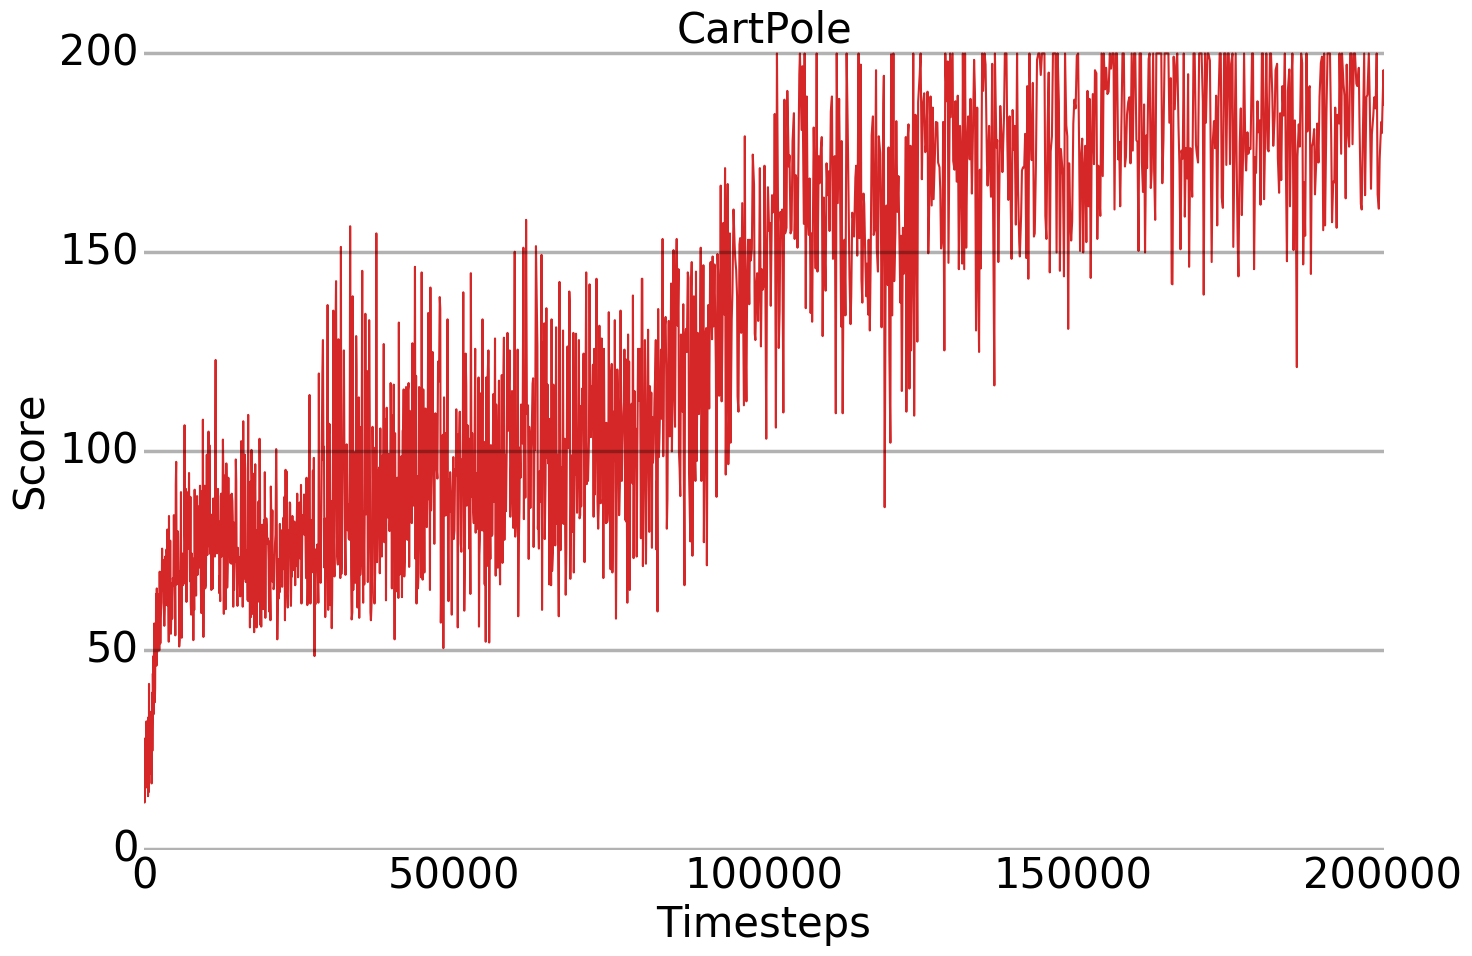
\includegraphics[width=0.95\textwidth]{plots/cartpole_2_threads.png}}
        \caption{A3C playing CartPole using 2 thread.}
        \label{cp:2}
    \end{subfigure}
  \end{tabular}
  \begin{tabular}[c]{cc}
    \begin{subfigure}[c]{.5\textwidth}
        \fbox{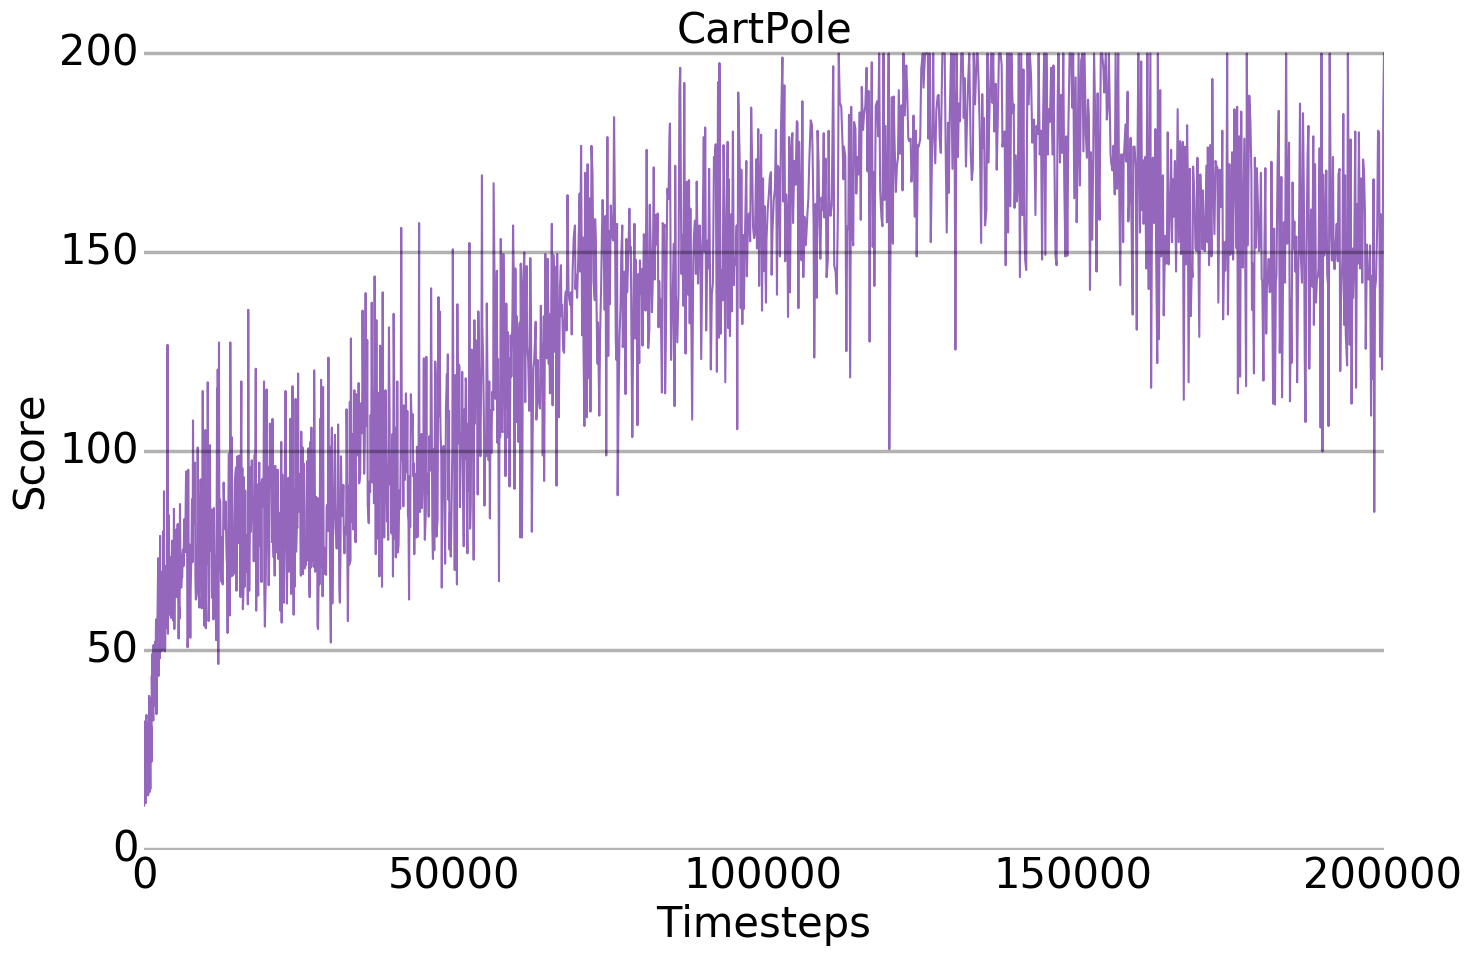
\includegraphics[width=0.95\textwidth]{plots/cartpole_4_threads.png}}
        \caption{A3C playing CartPole using 4 thread.}
        \label{cp:4}
    \end{subfigure}
    \begin{subfigure}[c]{.5\textwidth}
        \fbox{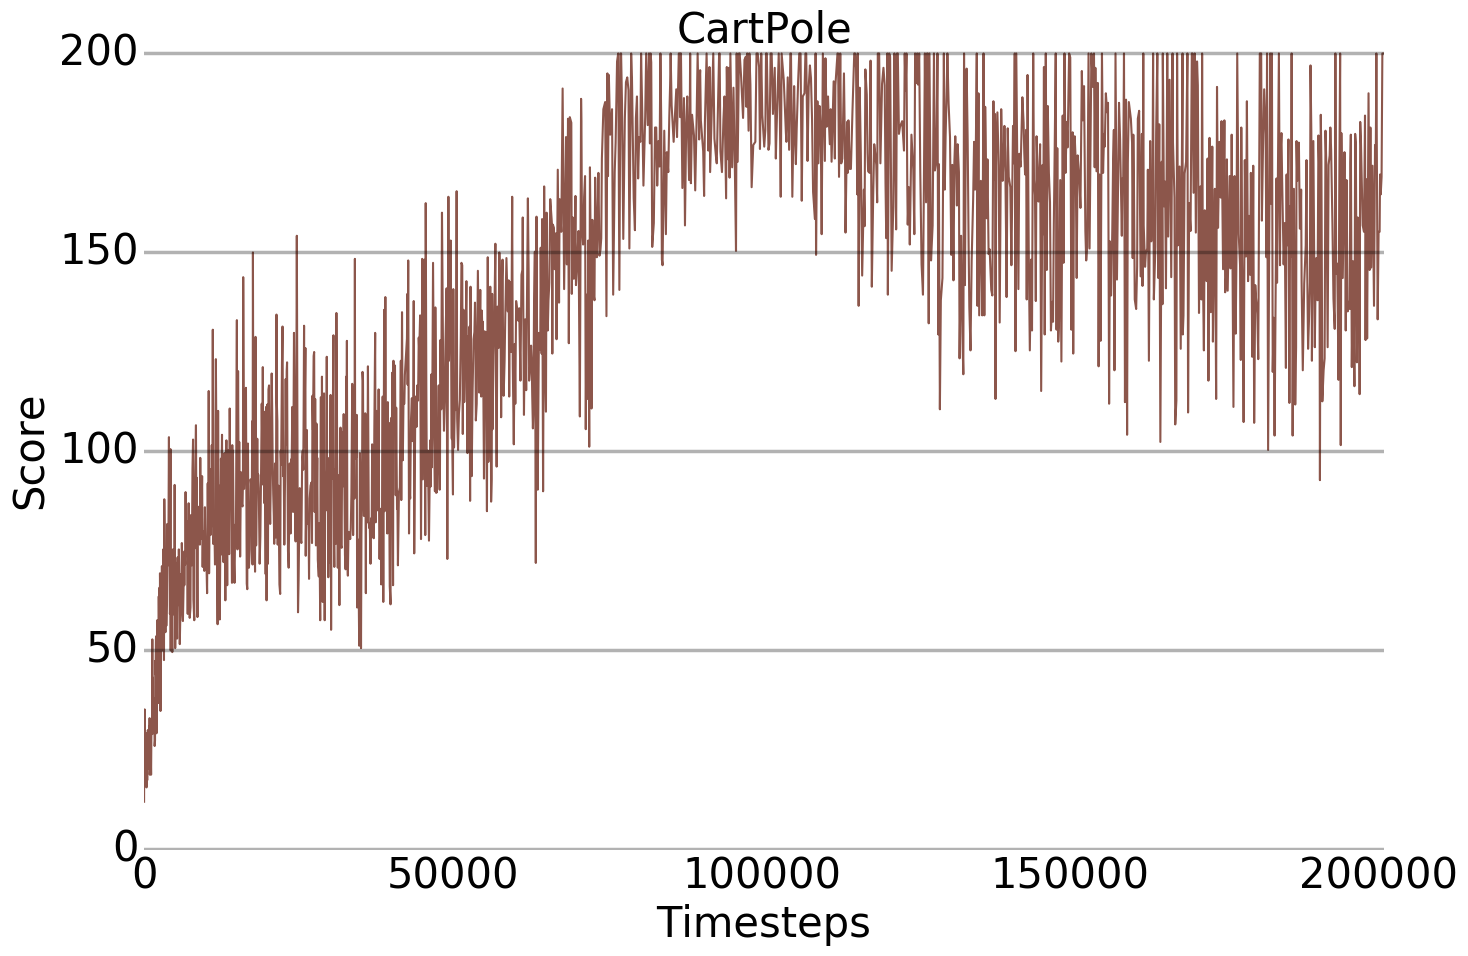
\includegraphics[width=0.95\textwidth]{plots/cartpole_8_threads.png}}
        \caption{A3C playing CartPole using 8 thread.}
        \label{cp:8}
    \end{subfigure}
  \end{tabular}
  \begin{tabular}[c]{c}
    \begin{subfigure}[c]{.5\textwidth}
        \fbox{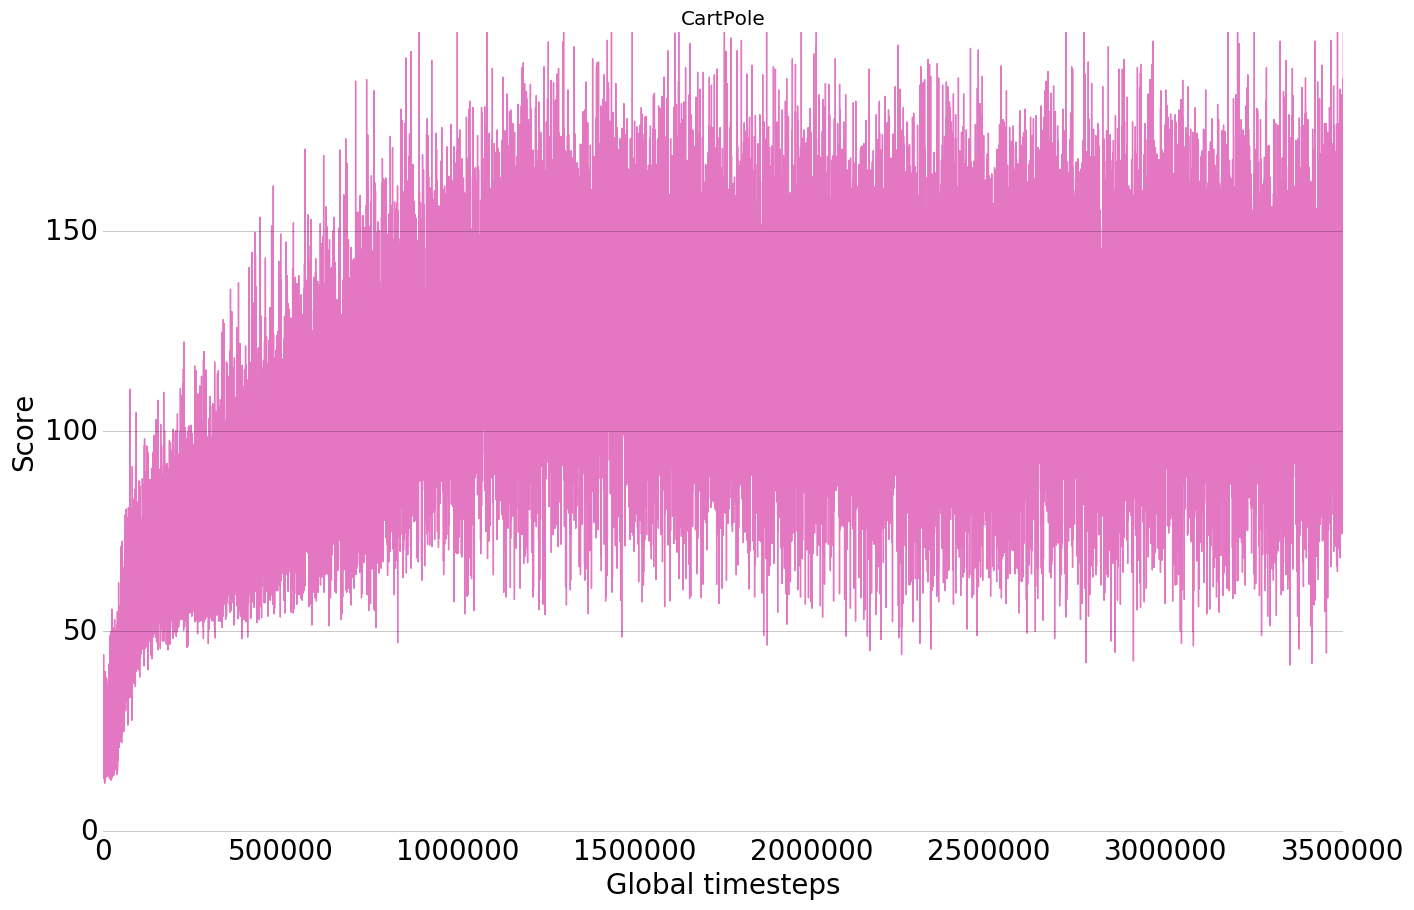
\includegraphics[width=0.95\textwidth]{plots/cartpole_16_threads.png}}
        \caption{A3C playing CartPole using 16 thread.}
        \label{cp:16}
    \end{subfigure}
  \end{tabular}
  \caption{The scores of all the different thread settings for the
    A3C implementation playing CartPole as a function of timesteps taken.}
     \label{fig:a3c_comp_steps}
\end{figure}

Upon closer inspectation of the results, it seems that the scores
converge at roughly the same pace.
It is again notable that the variance of the scores is approximately
the same for all thread settings, even though only the experiment using 16 threads
could maintain a stable mean score of 200.

\subsubsection{Comparison between A3C and Actor-Critic method using eligibility traces}

Figure \ref{fig:a3c_comp_eligibility} shows a comparison between the
results of the A3C algorithm and the Actor-Critic method with eligibility
traces.
The plots have been smoothed such that each point represents the mean score of the surrounding 50
points.

\begin{figure}[H]
    \centering
    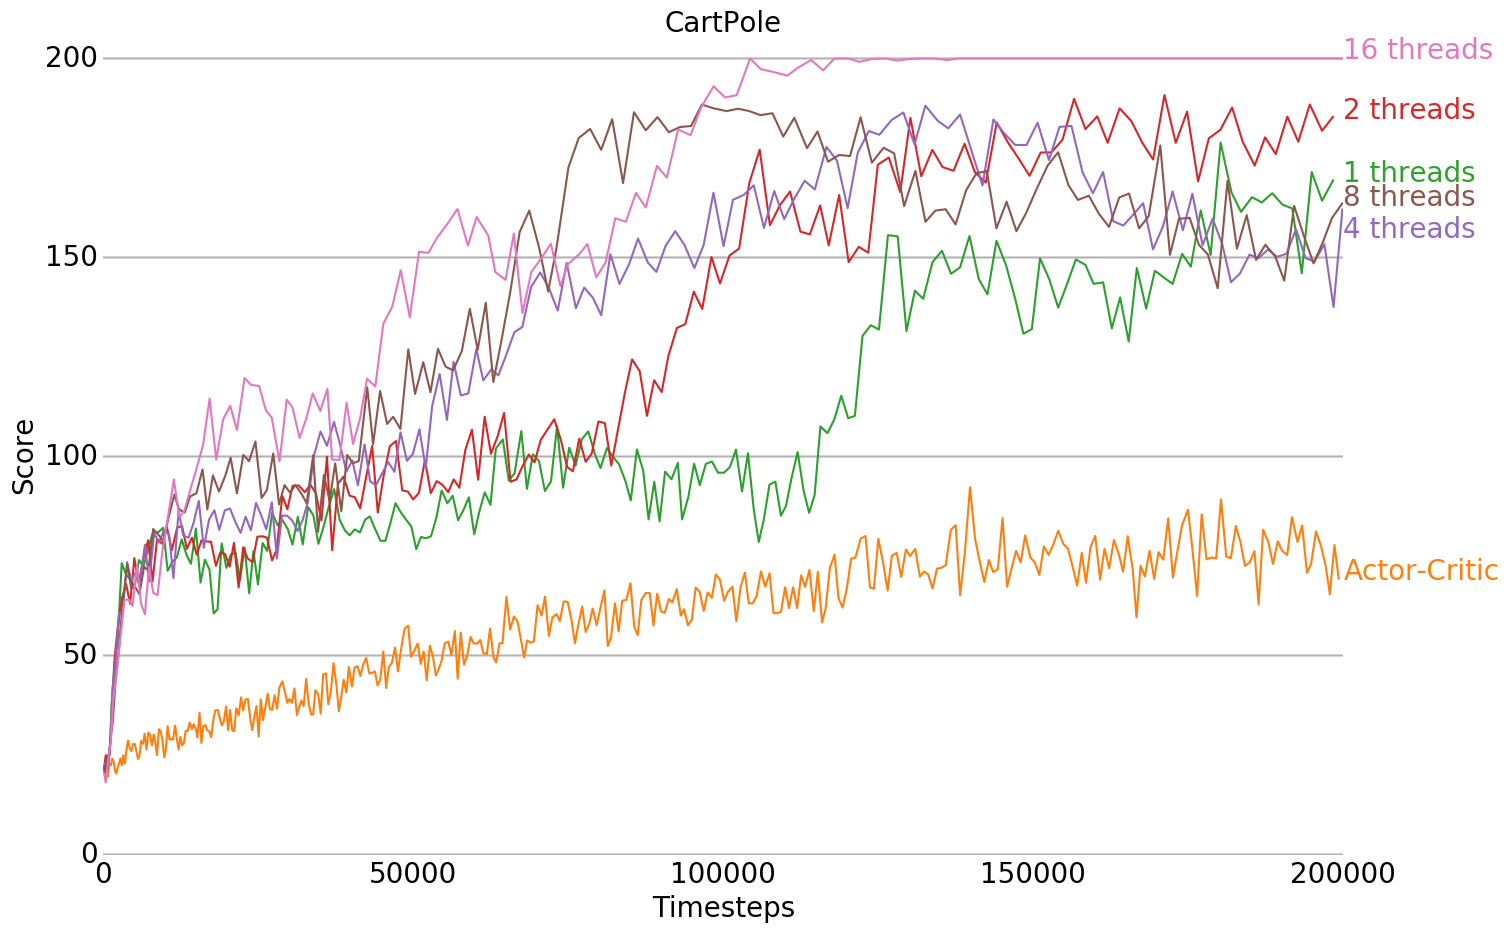
\includegraphics[scale=0.4]{plots/cartpole_compare_counter_with_AC.png}
    \caption{The results of the A3C algorithms different thread
            settings compared to the result of the Actor-Critic method
            with eligibility traces.}
    \label{fig:a3c_comp_eligibility}
\end{figure}

From the comparison it seems evident that the A3C algorithm is performing
better in regards to pace of learning and overall final mean for all thread settings.
However, the Actor-Critic with eligibity traces seem to present less variance
in its mean scores and learning curve.
Even using only a single thread, it seems that the A3C algorithm
is better suited for solving the CartPole problem, but it should
be kept in mind that the implementation of the Actor-Critic method
with eligibility traces was more restrained in regards to choice of
learning rates, which might be the reason why the learning happens
at such a low pace.

\subsection{Playing Atari games}

In the CartPole experiment we allowed our implementation to run for 200.000 timesteps.
However, due to the high amount of time required to
learn how to play Atari games, we have had to define the limit of the
Atari experiments based on the real time spent training.
The experiments were allowed to run for 16 hours (57.600 seconds)
for all thread settings, and only a single run was performed for
each of the games.
We have provided a brief overview of the results, for all games, in figure \ref{fig:all_atari},
which shows the scores as a function of real time spent for all
thread settings.
Each run completed between two and nine million timesteps.
To make the plots readable, they have been smoothed such that
each point represents the mean of the 500 surrounding points.

\begin{figure}[H]
  \begin{tabular}[c]{ccc}
    \begin{subfigure}[t]{.33\textwidth}
        \fbox{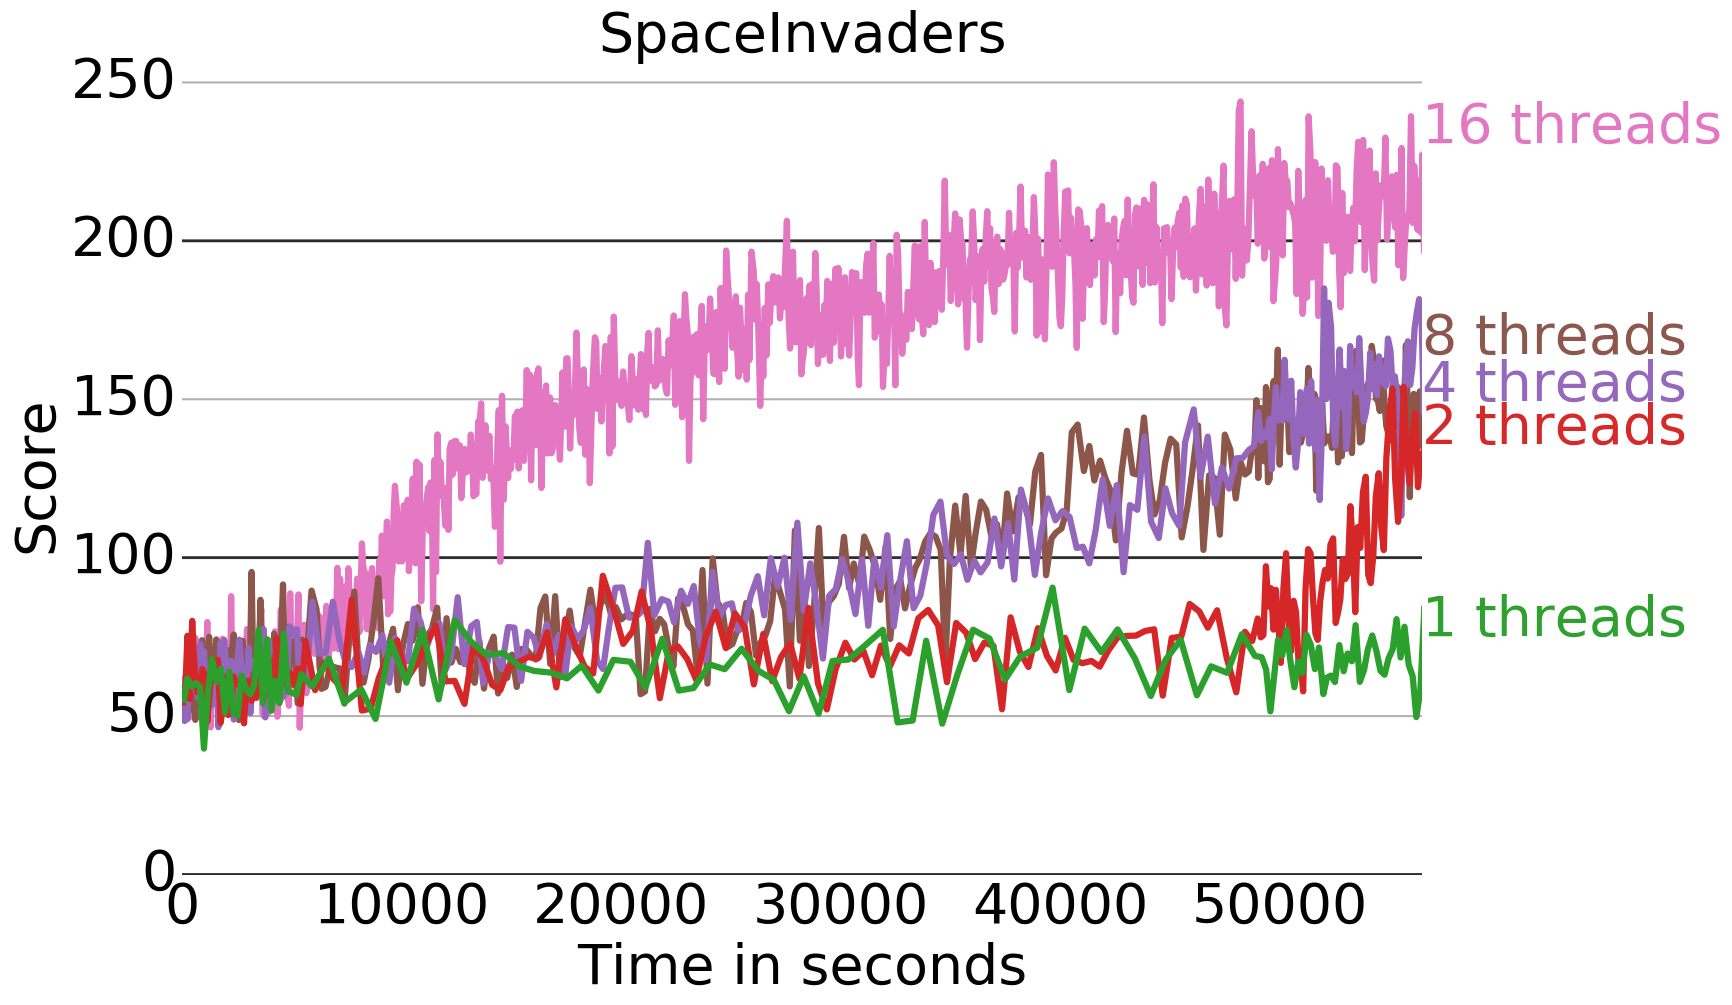
\includegraphics[width=.95\textwidth]{plots/spaceinvaders_intro_true.png}}
        \caption{Score achieved in Space Invaders as a function of
        consumed real-time.}
    \end{subfigure}
    \begin{subfigure}[t]{.33\textwidth}
        \fbox{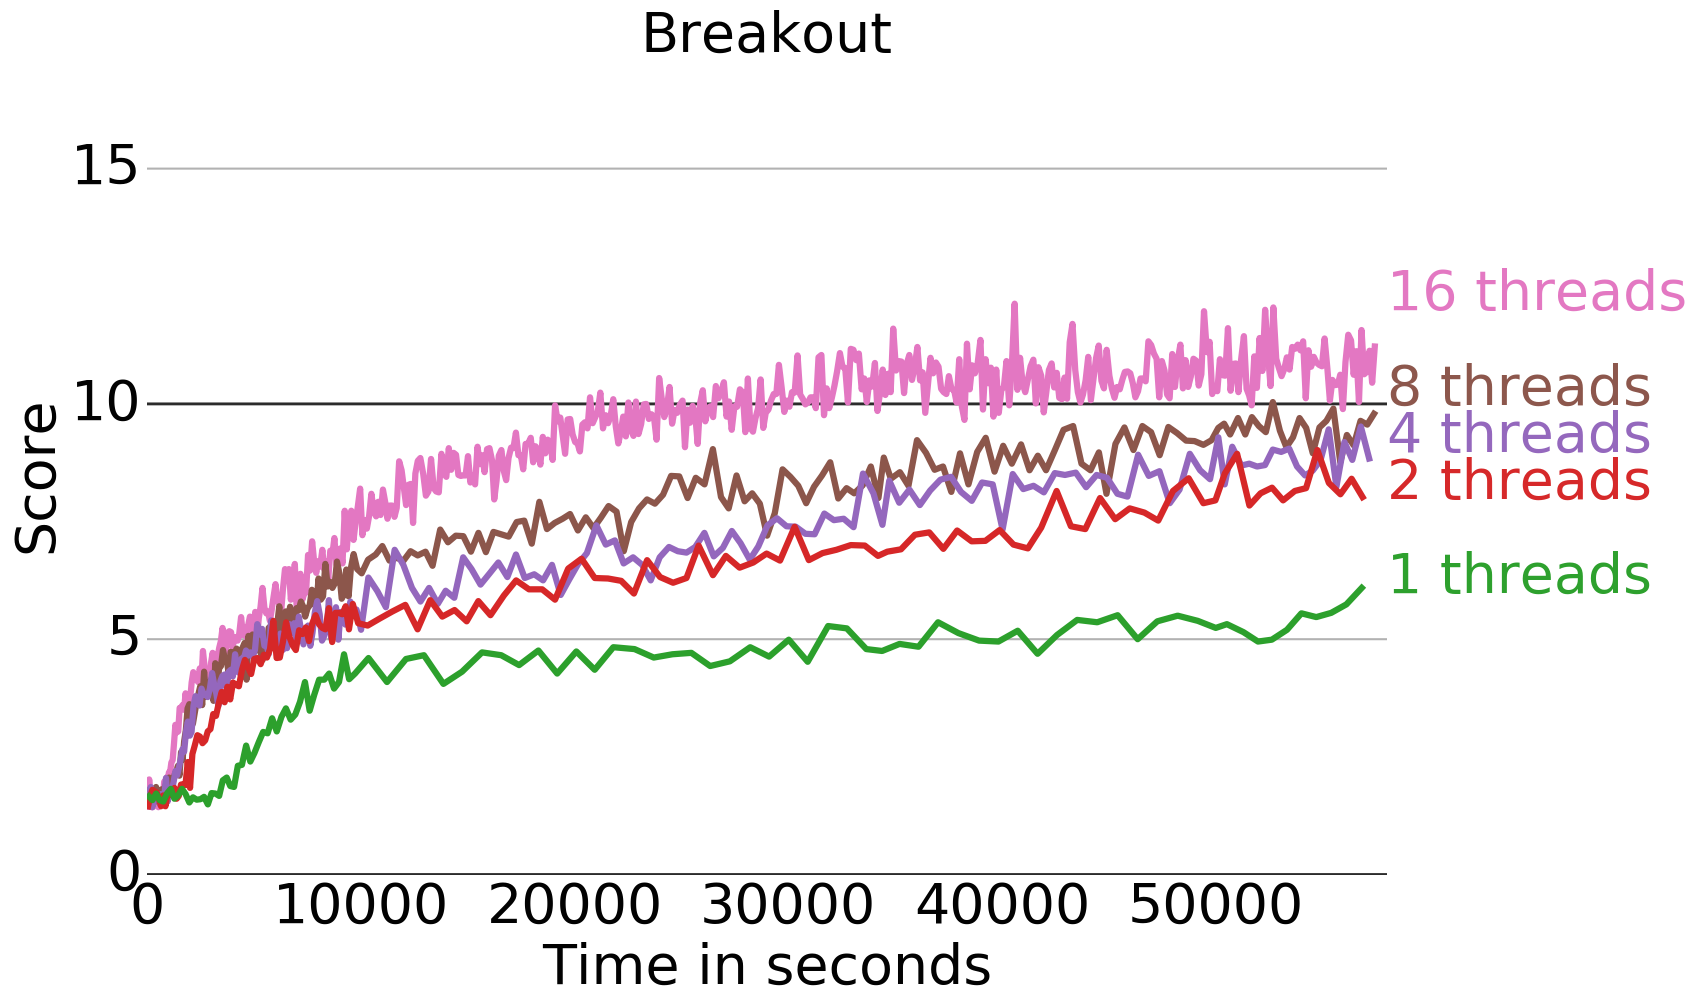
\includegraphics[width=.95\textwidth]{plots/breakout_intro.png}}
        \caption{Score achieved in Breakout as a function of
        consumed real-time.}
    \end{subfigure}
    \begin{subfigure}[t]{.32\textwidth}
        \fbox{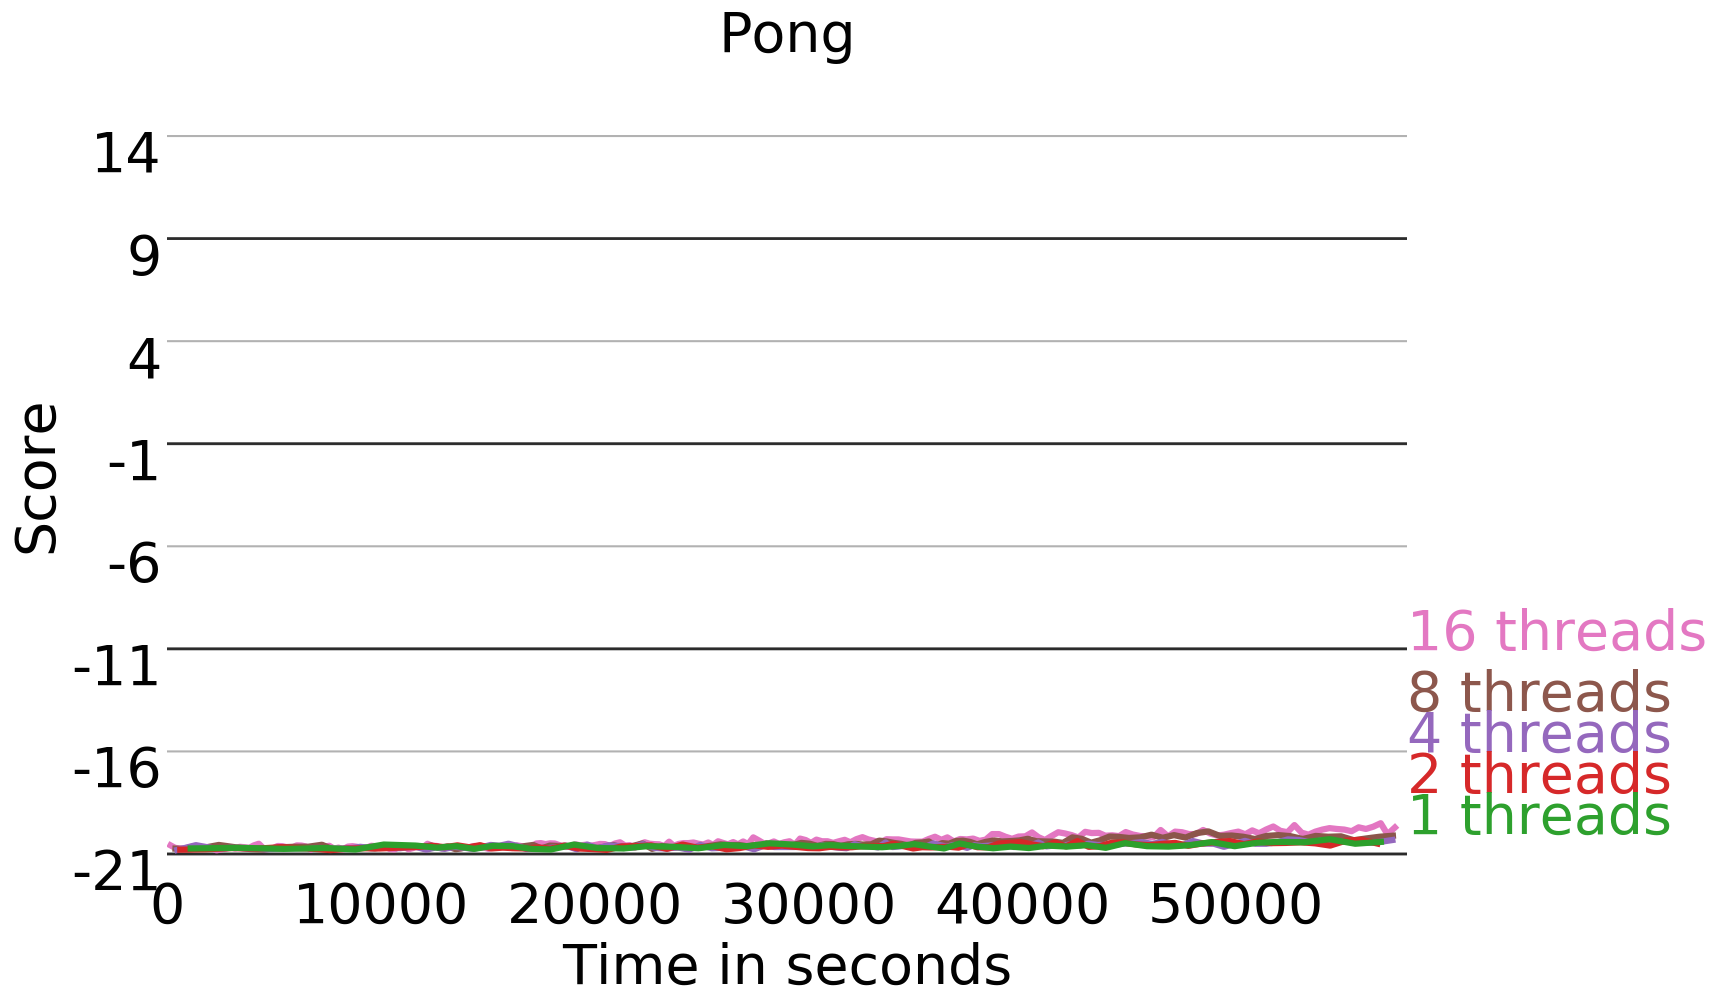
\includegraphics[width=.99\textwidth]{plots/pong_intro.png}}
        \caption{Score achieved in Pong as a function of
        consumed real-time.}
    \end{subfigure}
  \end{tabular}
  \label{fig:all_atari}
  \caption{Results for the three games the A3C algorithm have been used to play.}
\end{figure}

From these results it seems that the implementation is able to learn
a decent policy for both Space Invaders and Breakout, but fails
to learn how to play Pong.
Upon closer inspection, the results from Space Invaders seem to suggest
that a higher amount of threads, leads to a higher final mean score,
unlike the results from the CartPole experiments.
In figure \ref{fig:a3c_spaceinvaders} a view of the results from
playing Space Invaders with all the different thread settings is presented,
such that it is easier to see the finer differences.
The plot has been smoothed such that each point represents the mean of the
50 surrounding points.

\begin{figure}[H]
    \fbox{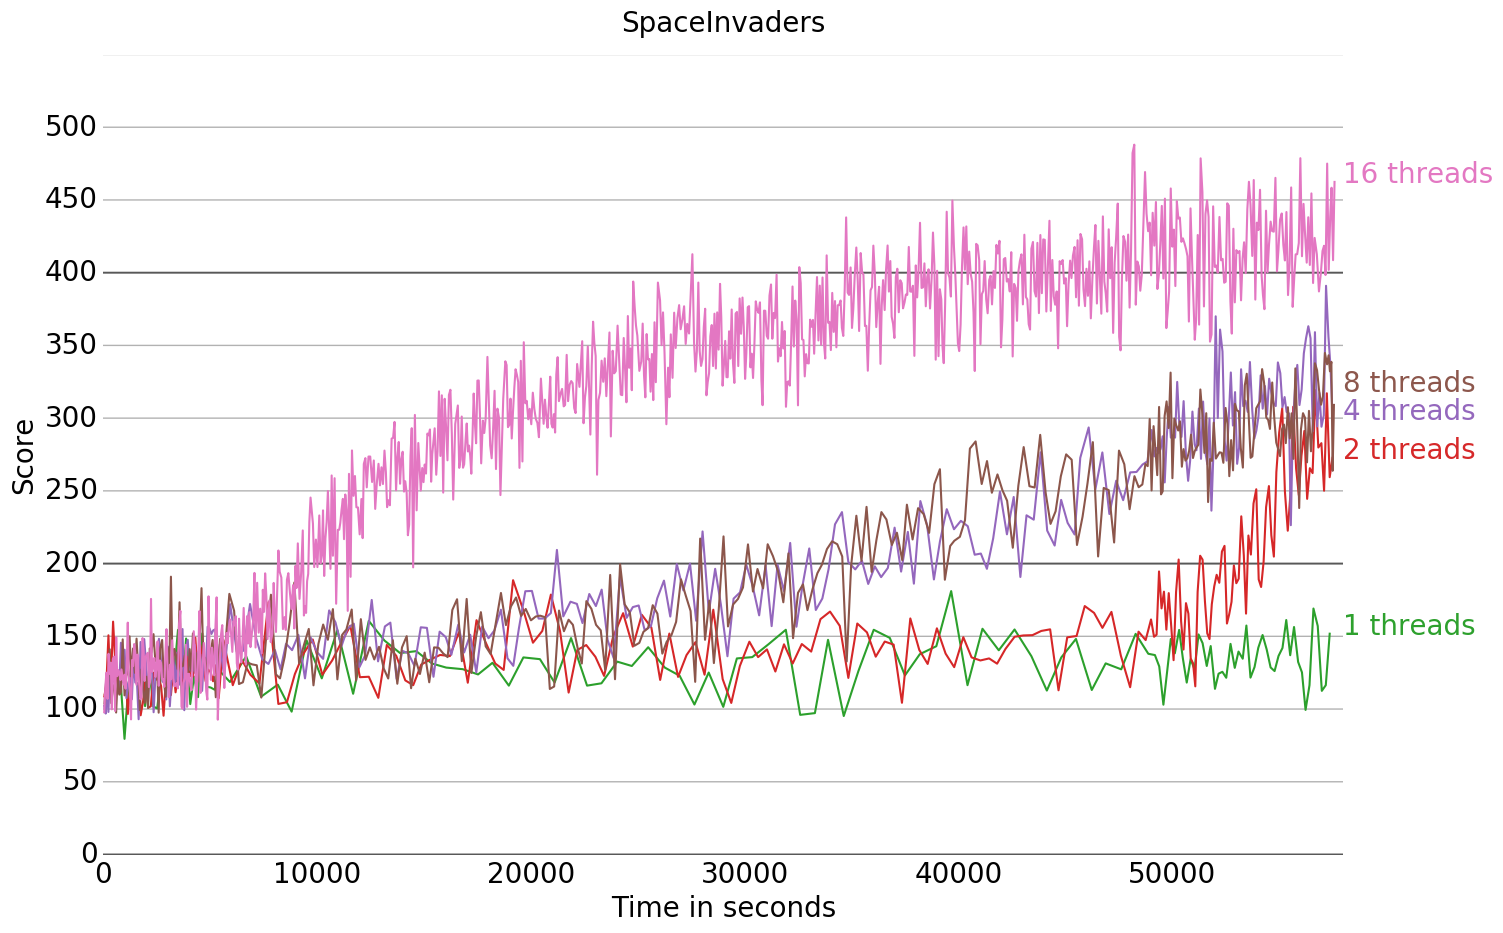
\includegraphics[width=.95\textwidth]{plots/spaceinvaders_compare_score_time.png}}
    \caption{Score achieved in Space Invaders as a function of
    consumed real-time.}
    \label{fig:a3c_spaceinvaders}
\end{figure}

Unlike the CartPole experiments with A3C, using multiple threads
actually lead to a higher learning pace.
This seems odd, but upon examining the amount of timesteps performed,
the result seems to make more sense.
Figure \ref{fig:a3c_spaceinvaders_ts} shows the same plot as
figure \ref{fig:a3c_spaceinvaders}, with the
exception that the score is a function of the timesteps taken
during the experiment.

\begin{figure}[H]
    \fbox{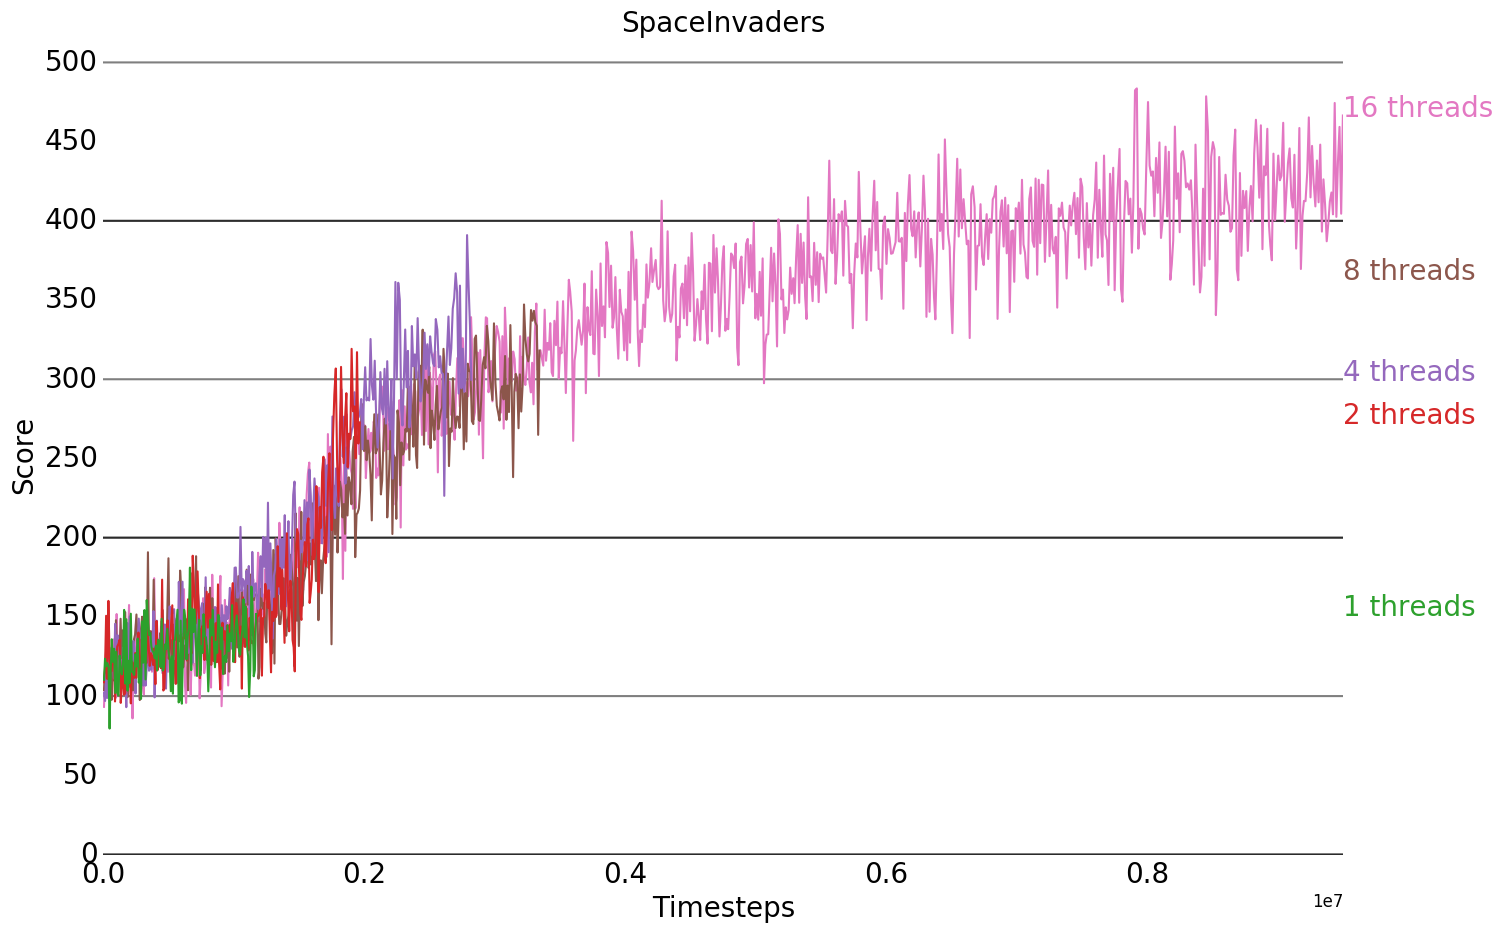
\includegraphics[width=.95\textwidth]{plots/spaceinvaders_score_timesteps.png}}
    \caption{Score achieved in Space Invaders as a function of
    timesteps taken.}
    \label{fig:a3c_spaceinvaders_ts}
\end{figure}

The plot suggests that the result of the A3C implementation
on Space Invaders behaves the same way as the results from the CartPole experiment,
if the threads are allowed to complete the same amount of timesteps.
This is the expected result, but it is notable that the amount
of completed timesteps doesn't seem to scale directly with
the amount of threads used.
It is especially curious that the difference in timesteps is very small
between four and eight threads, compared to the difference between sixteen and eight.
The same trend can be seen for Breakout, which is shown in figure
\ref{fig:a3c_breakout_comp}.

\begin{figure}[H]
  \centering   
  \begin{tabular}[c]{cc}
    \begin{subfigure}[c]{.5\textwidth}
        \fbox{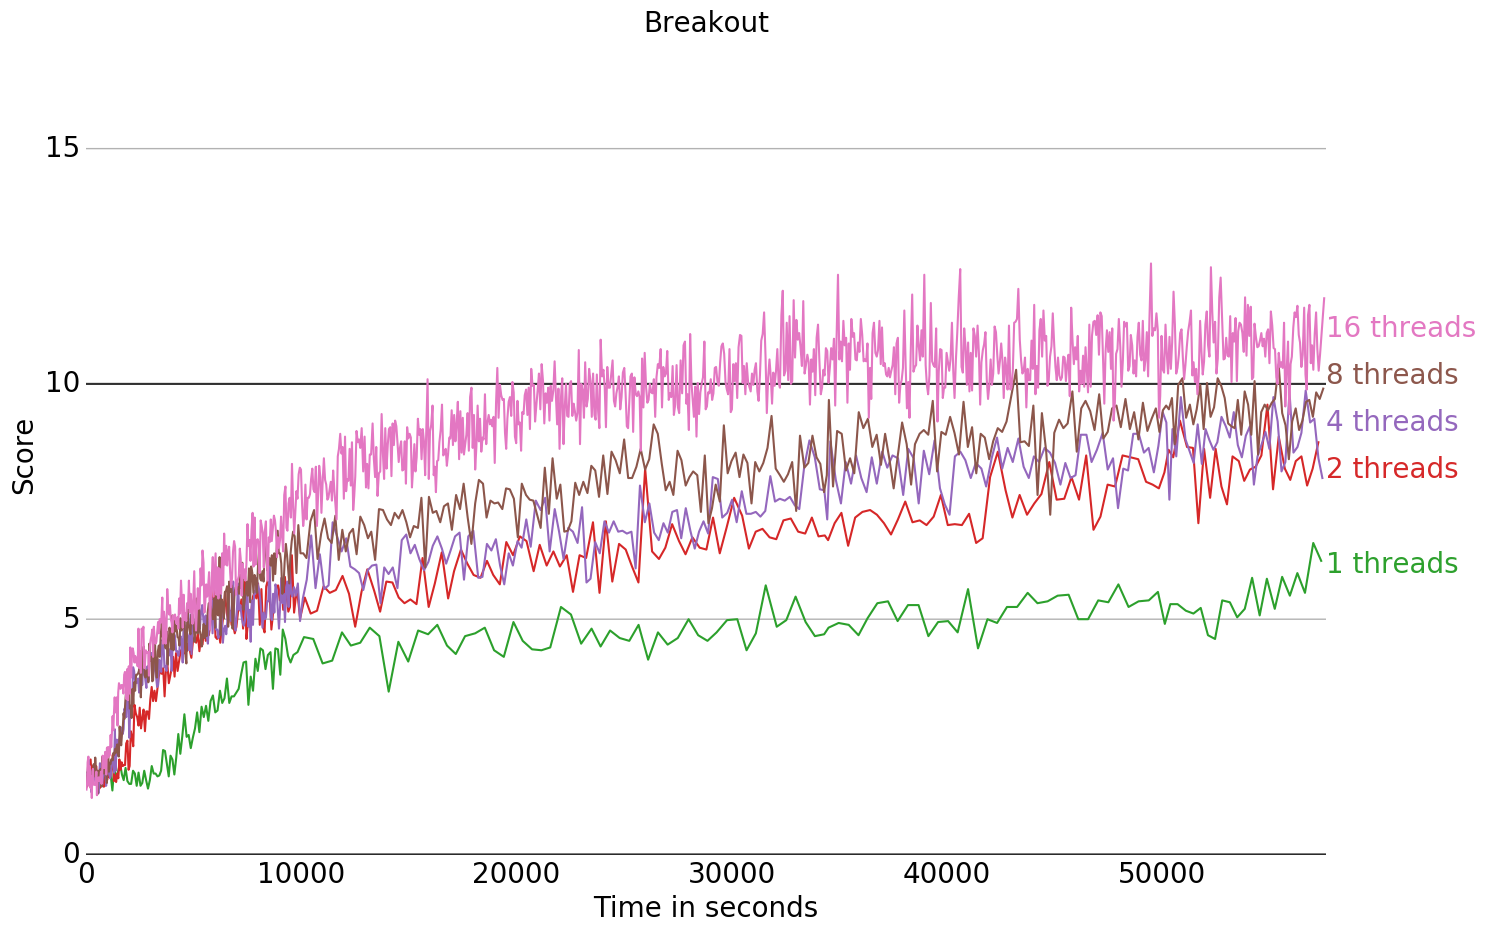
\includegraphics[width=0.97\textwidth]{plots/breakout_compare_time.png}}

        \caption{Score achieved in Breakout as a function of consumed real-time.}
    \end{subfigure}
    \begin{subfigure}[c]{.5\textwidth}

        \fbox{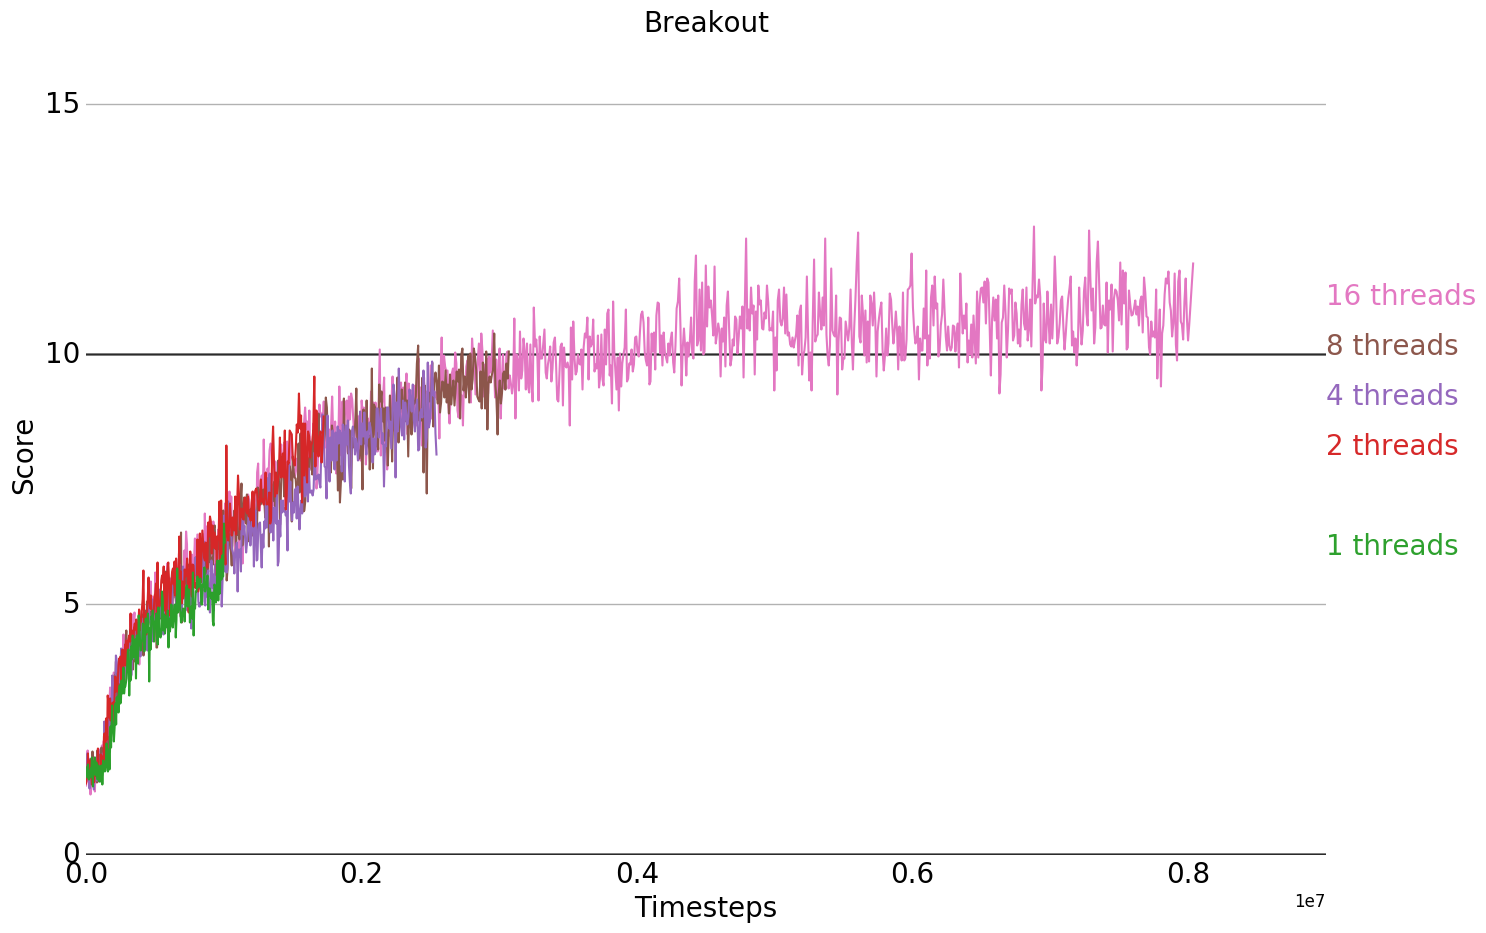
\includegraphics[width=0.97\textwidth]{plots/breakout_steps.png}}
        \caption{Score achieved in Breakout as a function of 
        timesteps taken.}
    \end{subfigure}
  \end{tabular}
  \caption{The scores of all the different thread settings for the
    A3C implementation playing Breakout. The plot has been smoothed, which means every
point describes the mean of the surrounding 50.}
     \label{fig:a3c_breakout_comp}
\end{figure}

These results reinforce the idea that the A3C algorithm is behaving
the same way as it did for the CartPole experiments, with the exception
that we are able to complete a lot more timesteps 
in the Atari games for each additional thread used.

We have also tested our A3C implementation on the Pong enviroment.
The setup of the training was the same as for the Breakout and Spaceinvaders experiments,
but as shown below the results difer significantly in regards
to improvement of the mean score. 

\begin{figure}[H]
  \centering   
  \begin{tabular}[c]{cc}
    \begin{subfigure}[c]{.5\textwidth}
        \fbox{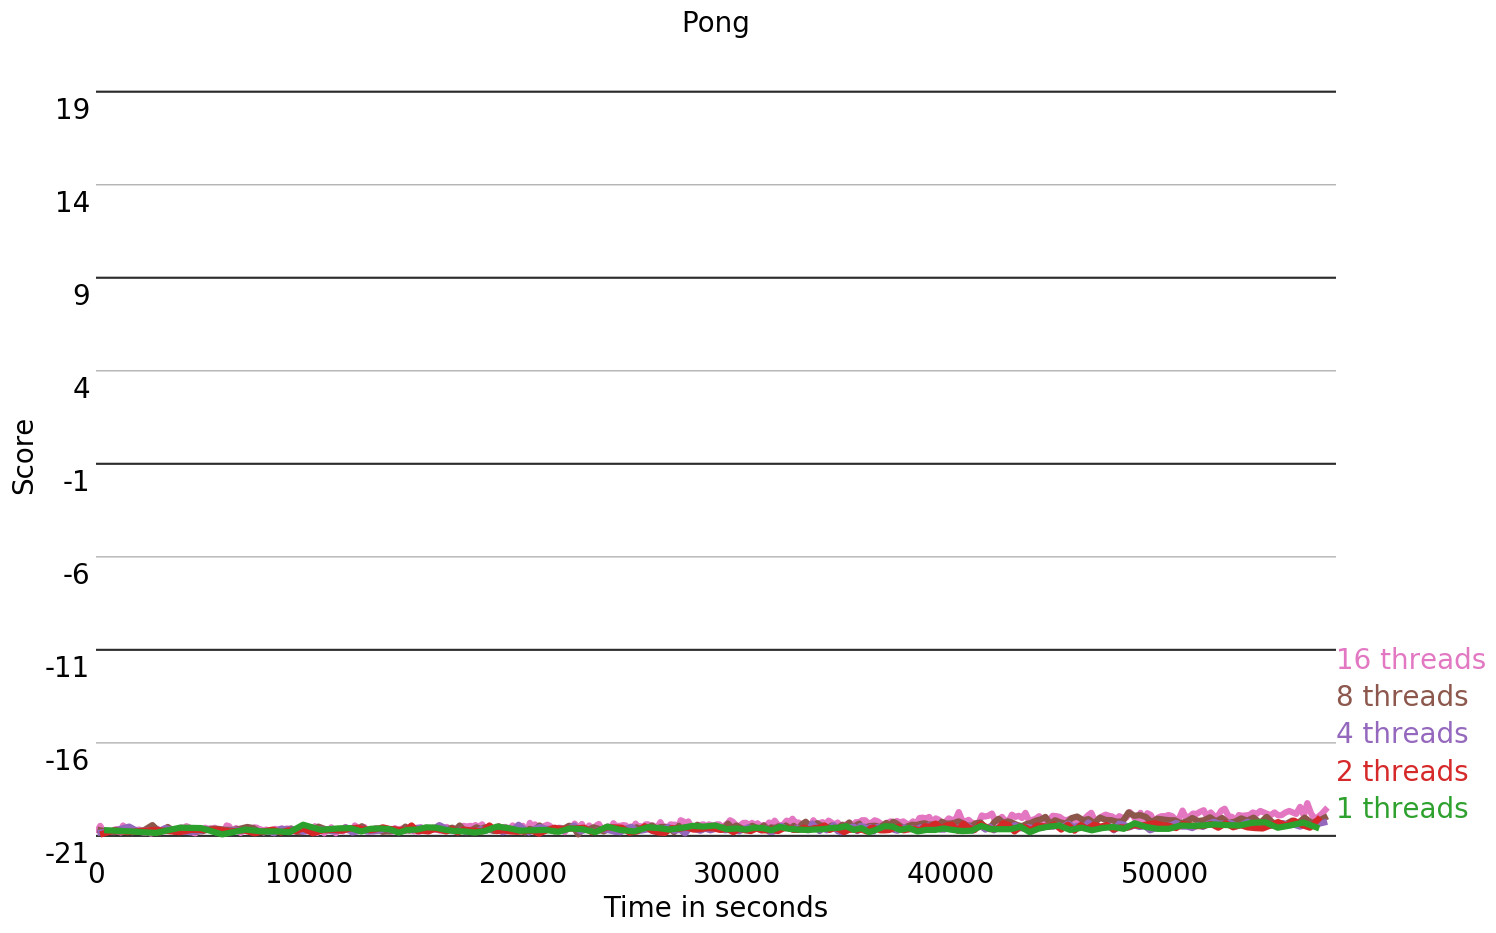
\includegraphics[width=0.97\textwidth]{plots/pong_time.png}}

        \caption{Score achieved in Pong as a function of consumed real-time.}
    \end{subfigure}
    \begin{subfigure}[c]{.5\textwidth}

        \fbox{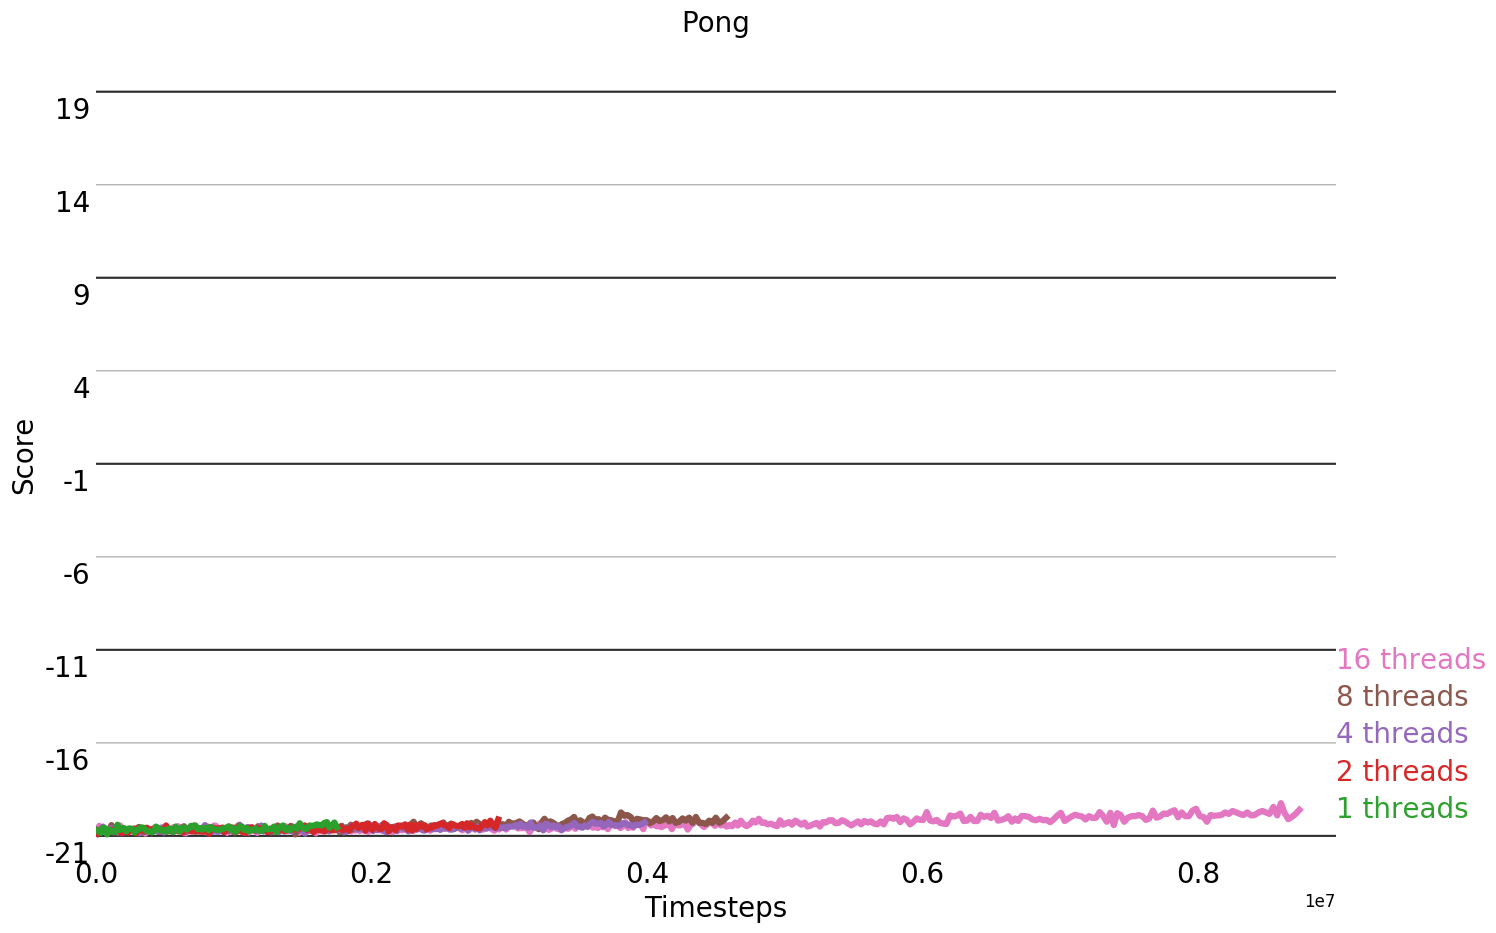
\includegraphics[width=0.97\textwidth]{plots/pong_steps.png}}
        \caption{Score achieved in Pong as a function of 
        timesteps taken.}
    \end{subfigure}
  \end{tabular}
  \caption{The scores of all the different thread settings for the
    A3C implementation playing Pong. 
The plot has been smoothed, which means every
point describes the mean of the surrounding 50.}
     \label{fig:a3c_pong_comp}
\end{figure}

Generally, we see no improvement in performance while playing Pong for any of the threads settings.
Upon closer examination it seems that the experiment using 16 threads improves a little
in the end, but it is too small a change to conclude that the method learned to play the 
game.
However, with regards to the number of timesteps completed,
the trend is the same as the one in the Breakout and Space Invaders experiments.

We have seen some varying results from the different experiments, with
the most notable result being that the advantages of using multiple threads in the A3C method
seems to only be present in the Atari experiments.
We expected the results for the Actor-Critic method using eligibility traces
to be worse than those generated by the A3C experiments, 
but the difference was more prominent than expected.

\end{document}
